\begin{center}
  \Large
  \textbf{BIOGRAFI PENULIS}
\end{center}

\addcontentsline{toc}{chapter}{BIOGRAFI PENULIS}

\vspace{2ex}

\begin{wrapfigure}{L}{0.3\textwidth}
  \centering
  \vspace{-3ex}
  % Ubah file gambar berikut dengan file foto dari mahasiswa
  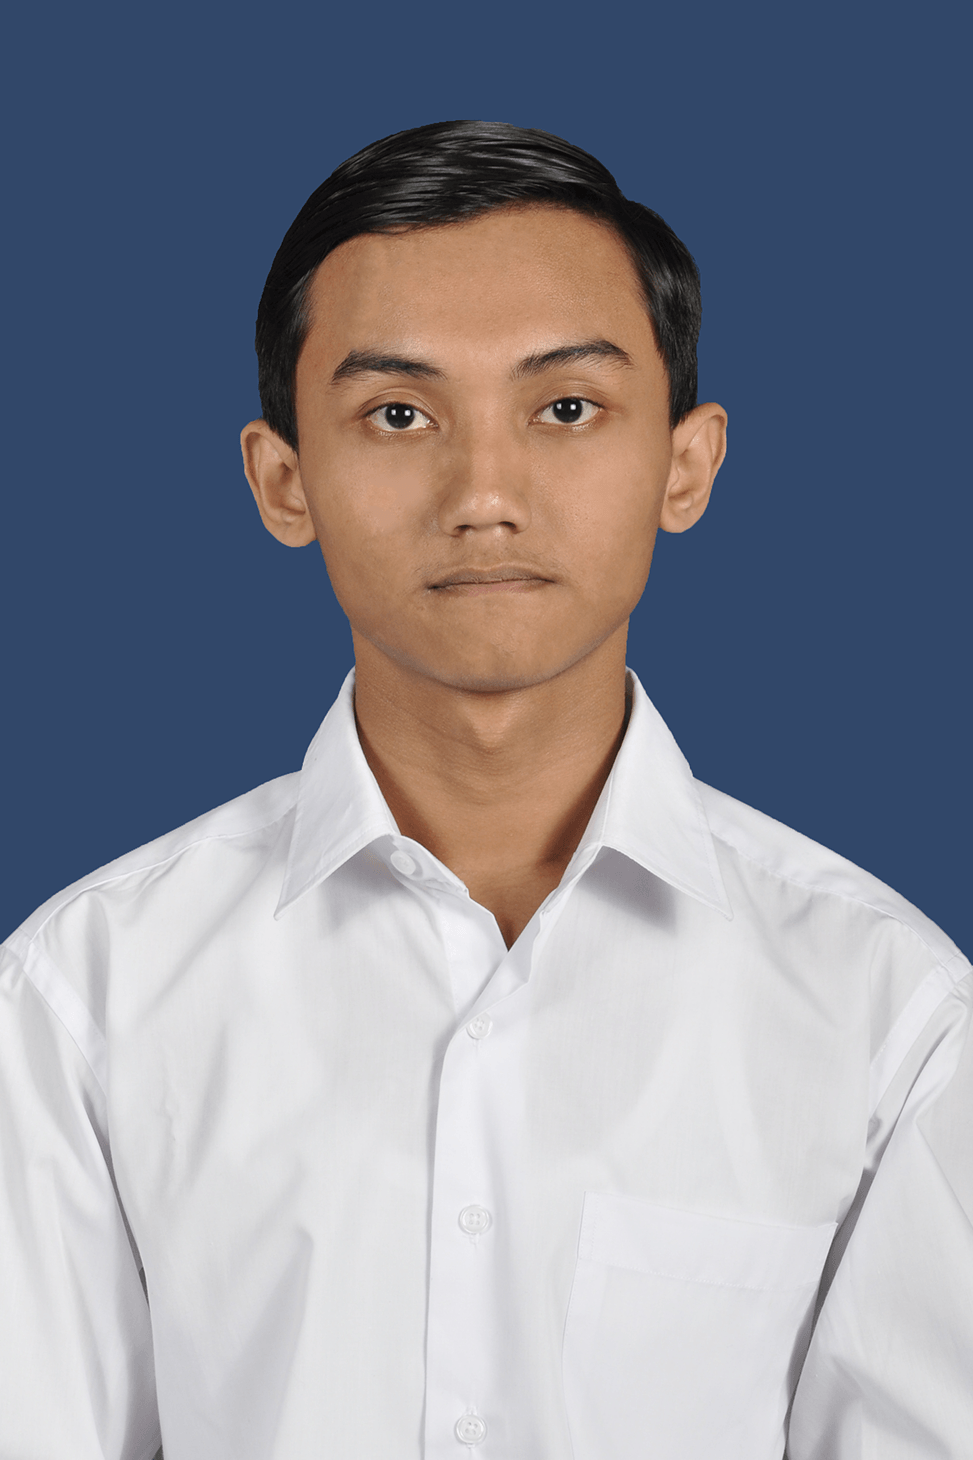
\includegraphics[width=0.3\textwidth]{gambar/foto diri.png}
  \vspace{-4ex}
\end{wrapfigure}

% Ubah kalimat berikut dengan biografi dari mahasiswa
\name{}, lahir di kota kecil bernama Pati pada tanggal 2 Januari 2002. Lahir sebagai anak pertama dari dua bersaudara. Satrio memulai pendidikannya di TK PGRI Sumbermulyo, kemudian melanjutkan pendidikan di SD Sumbermulyo 03. Pada kelas 4, SD ini memiliki murid terlalu sedikit sehingga harus diberhentikan operasionalnya. Satrio memutuskan untuk pindah ke SD Sumbermulyo 02, yang mana lebih dekat jaraknya ke rumahnya. Setelah lulus dari SD, satrio melanjutkan pendidikannya ke SMP Negeri 1 Pati. Hal ini berbeda dengan kebanyakan teman sekelasnya yang memilih untuk melanjutkan ke SMP di daerah winong ataupun Gabus. Satrio menjadi satu-satunya murid dari desanya yang bersekolah di SMPN 1 Pati kala itu.  \lipsum[1-3]